\documentclass[10pt,a4paper]{article}
\usepackage[T1]{fontenc}
\usepackage[utf8]{inputenc}
\usepackage[expansion=false]{microtype}
\usepackage{lmodern}
\usepackage[a4paper, top=14mm, bottom=14mm, left=18mm, right=18mm]{geometry}
\usepackage{amsmath,amssymb}
\usepackage{xcolor}
\usepackage{tikz}
\usetikzlibrary{arrows.meta,positioning,calc}
\usepackage{booktabs}
\usepackage{enumitem}
\usepackage{multicol}
\usepackage{titlesec}
\usepackage[hidelinks]{hyperref}
\usepackage{array}

\definecolor{thesisblue}   {RGB}{0,  70, 140}
\definecolor{thesisgreen}  {RGB}{ 20,120,  60}
\definecolor{thesisgray}   {RGB}{100,100, 110}
\definecolor{lightblue}    {RGB}{220,235,255}
\definecolor{lightgreen}   {RGB}{220,245,225}

\newcommand{\kibr}{k_{\mathrm{ibr}}}
\newcommand{\Zline}{Z_{\mathrm{line}}}
\newcommand{\ZL}{Z_L}
\newcommand{\ZF}{Z_F}

\titleformat{\section}{\small\bfseries\color{thesisblue}}{}{0em}{}
  [\vspace{-5pt}\textcolor{thesisblue!35}{\rule{\linewidth}{0.4pt}}\vspace{1pt}]
\titlespacing{\section}{0pt}{6pt}{2pt}
\setlength{\parskip}{2pt}
\setlength{\parindent}{0pt}

\begin{document}
\pagestyle{empty}

%% Title
\noindent
{\LARGE\bfseries\color{thesisblue} SAMBPS}\enspace
{\large Self-Adaptive Model-Based Protection Systems}
\hfill{\small\itshape\color{thesisgray}PhD Thesis --- one-page overview}\\[-2pt]
{\small\color{thesisgray}A hierarchical, physics-aware relay architecture for inverter-rich distribution networks.}

\vspace{1pt}\textcolor{thesisblue!30}{\rule{\linewidth}{0.8pt}}\vspace{3pt}

%% Section 1
\section{Why a New Protection Architecture?}

\small
Classical protection relays rest on three assumptions that held for synchronous-generator networks:
fault current is \emph{large} (6--10\,pu), \emph{passive} (determined by physics, not software), and
\emph{directionally predictable} in radial feeders.
Inverter-Based Resources (IBRs) violate all three: fast current control caps fault current at
1.1--2.0\,pu within 2--5\,ms; its magnitude, phase, and sequence composition are set by firmware;
and distributed IBRs at every node make feeders bidirectional and meshed.
The result is systematic failure of legacy overcurrent, distance, and differential relays ---
a \emph{protection crisis} worsening as IBR penetration approaches 70--80\% of new capacity by 2030.
SAMBPS replaces fixed-setting relays with a two-tier adaptive scheme informed by a real-time digital twin.

\vspace{3pt}

%% Section 2 — TikZ
\section{Two-Tier Architecture}

\vspace{2pt}\noindent
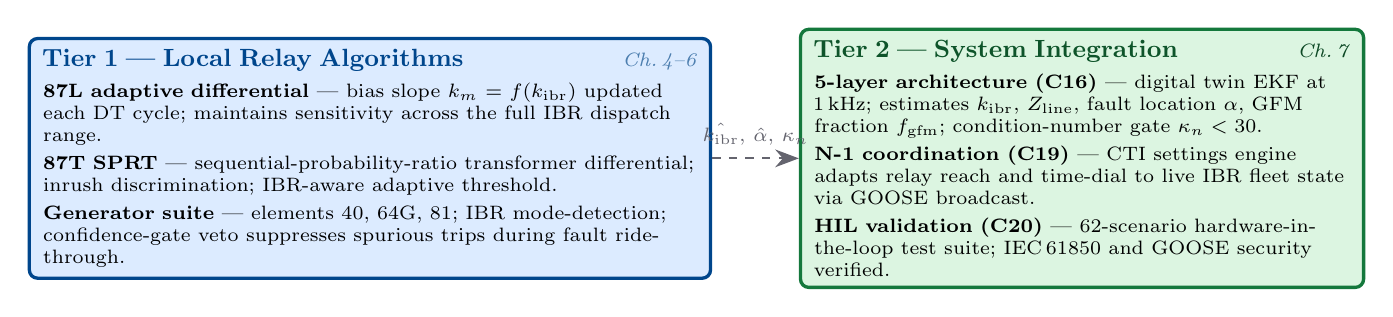
\begin{tikzpicture}[every node/.style={font=\scriptsize}]

\node[draw=thesisblue, very thick, rounded corners=3pt,
      fill=lightblue, text width=8.3cm, align=left,
      inner xsep=5pt, inner ysep=4pt] (T1) at (0,0) {%
  {\small\textbf{\color{thesisblue}Tier~1 --- Local Relay Algorithms}}%
  \hfill{\itshape\color{thesisblue!70}Ch.\,4--6}\\[3pt]
  \textbf{87L adaptive differential} --- bias slope $k_m\!=\!f(\kibr)$ updated each DT
  cycle; maintains sensitivity across the full IBR dispatch range.\\[2pt]
  \textbf{87T SPRT} --- sequential-probability-ratio transformer differential;
  inrush discrimination; IBR-aware adaptive threshold.\\[2pt]
  \textbf{Generator suite} --- elements 40, 64G, 81; IBR mode-detection;
  confidence-gate veto suppresses spurious trips during fault ride-through.};

\node[draw=thesisgreen, very thick, rounded corners=3pt,
      fill=lightgreen, text width=6.8cm, align=left,
      inner xsep=5pt, inner ysep=4pt,
      right=1.1cm of T1] (T2) {%
  {\small\textbf{\color{thesisgreen!70!black}Tier~2 --- System Integration}}%
  \hfill{\itshape\color{thesisgreen!60!black}Ch.\,7}\\[3pt]
  \textbf{5-layer architecture (C16)} --- digital twin EKF at 1\,kHz;
  estimates $\kibr$, $\Zline$, fault location $\alpha$,
  GFM fraction $f_{\mathrm{gfm}}$; condition-number gate $\kappa_n<30$.\\[2pt]
  \textbf{N-1 coordination (C19)} --- CTI settings engine adapts relay reach
  and time-dial to live IBR fleet state via GOOSE broadcast.\\[2pt]
  \textbf{HIL validation (C20)} --- 62-scenario hardware-in-the-loop test
  suite; IEC\,61850 and GOOSE security verified.};

\draw[-{Stealth[length=3mm]}, dashed, thick, thesisgray]
  (T1.east) --
  node[above, yshift=1pt, font=\scriptsize, thesisgray]
    {$\hat{\kibr},\,\hat{\alpha},\,\kappa_n$}
  (T2.west);

\end{tikzpicture}

\vspace{3pt}

%% Section 3 — Problems table
\section{Four Problems Addressed}

\small\renewcommand{\arraystretch}{1.22}
\begin{tabular}{@{} >{\bfseries}p{0.3cm} p{3.0cm} p{12.1cm} @{}}
\toprule
 & \textbf{Problem} & \textbf{What fails \;/\; SAMBPS fix} \\
\midrule
P1 & 87L threshold failure &
  Fixed $k_m$ is too conservative at low $\kibr$ (misses high-impedance faults)
  and too permissive at high $\kibr$ (false restrain during FRT).
  \textit{Fix:} $k_m = f(\kibr)$ from the 5-layer model, updated every DT cycle. \\
P2 & Distance under-reach &
  IBR current limiting inflates apparent impedance
  $Z_{\mathrm{app}} = \alpha Z_L + \tfrac{I_A+I_B}{I_A}Z_F > \alpha Z_L$;
  relay under-reaches beyond 60--70\% of line.
  \textit{Fix:} IBR-aware quadrilateral characteristic with online reach correction
  using $\hat{\kibr}$. \\
P3 & Microgrid mode transition &
  50--200\,ms gap between grid-connected and islanded modes leaves no valid
  setting group.
  \textit{Fix:} mode-triggered setting-group pre-arming synchronised via GOOSE
  before the transfer. \\
P4 & No real-time IBR visibility &
  Settings computed offline for a fixed fleet; $\kibr$ varies continuously with
  irradiance and curtailment.
  \textit{Fix:} digital twin EKF tracks $\kibr$, $\Zline$, $\alpha$ at 1\,kHz;
  trusted when $\kappa_n < 30$. \\
\bottomrule
\end{tabular}

\vspace{3pt}

%% Section 4 — Key results
\section{Key Results}

\small
\begin{multicols}{3}
\begin{itemize}[leftmargin=1em, itemsep=1pt, topsep=0pt]
  \item \textbf{95.8\%} DT--relay agreement\\(N\,=\,2\,000 MC, Study\,E)
  \item \textbf{0\%} FLAG\_FP / FLAG\_FN\\in 87L and Z1 regions
  \item \textbf{28.5$\times$} $\kibr$ RMSE gain\\with phasor-DFT EKF
  \item \textbf{52\,ms} fault clearance;\\DT adds \textbf{0\,ms} latency
  \item \textbf{62 HIL scenarios} passed;\\all N-1 contingencies cleared
  \item $\kappa_n < 30$ gate trusted\\in \textbf{97.3\%} of events
\end{itemize}
\end{multicols}

\vspace{2pt}\textcolor{thesisblue!25}{\rule{\linewidth}{0.4pt}}
{\footnotesize\color{thesisgray}
\textbf{Reproduce:}~\texttt{python -m sambp.digital\_twin.run\_dt\_lab --study E --n-mc 2000}
\quad\textbar\quad Tag:~\texttt{sambp-dt-lab-v0.1}
\quad\textbar\quad Supersedes TR-43/44/45 standalone scripts.}

\end{document}
